\section{Ordenacao e ordenação invertida}
Todos os algoritmos e suas variações estão implementados no codigo a seguir. 
\lstinputlisting{../ex11/ordenacao.c}
\begin{figure}[h!]
	\centering
	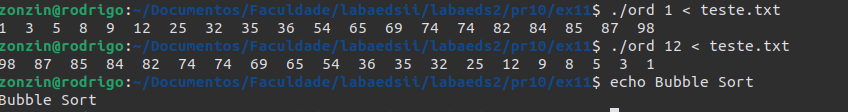
\includegraphics[width=0.7\linewidth]{imgs/bubble}
	\caption{Bubble Sort}
	\label{fig:bubble}
\end{figure}

\begin{figure}[h!]
	\centering
	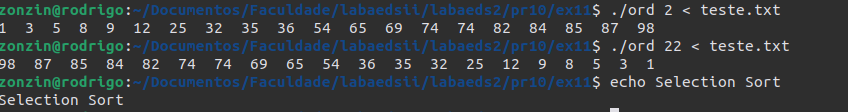
\includegraphics[width=0.7\linewidth]{imgs/selec}
	\caption{Selection Sort}
	\label{fig:selec}
\end{figure}

\begin{figure}[h!]
	\centering
	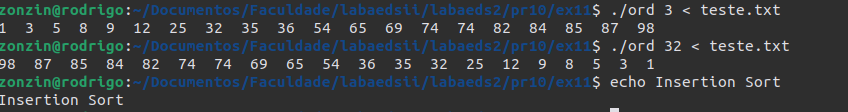
\includegraphics[width=0.7\linewidth]{imgs/insertion}
	\caption{Insertion Sort}
	\label{fig:insertion}
\end{figure}


\section{Complexidade - deu errado}
Por algum motivo, o comportamento assintótico não está sendo observado em nenhum dos plots. Em razão do horário (23h37), eu desisto. 

\begin{figure}[h!]
	\centering
	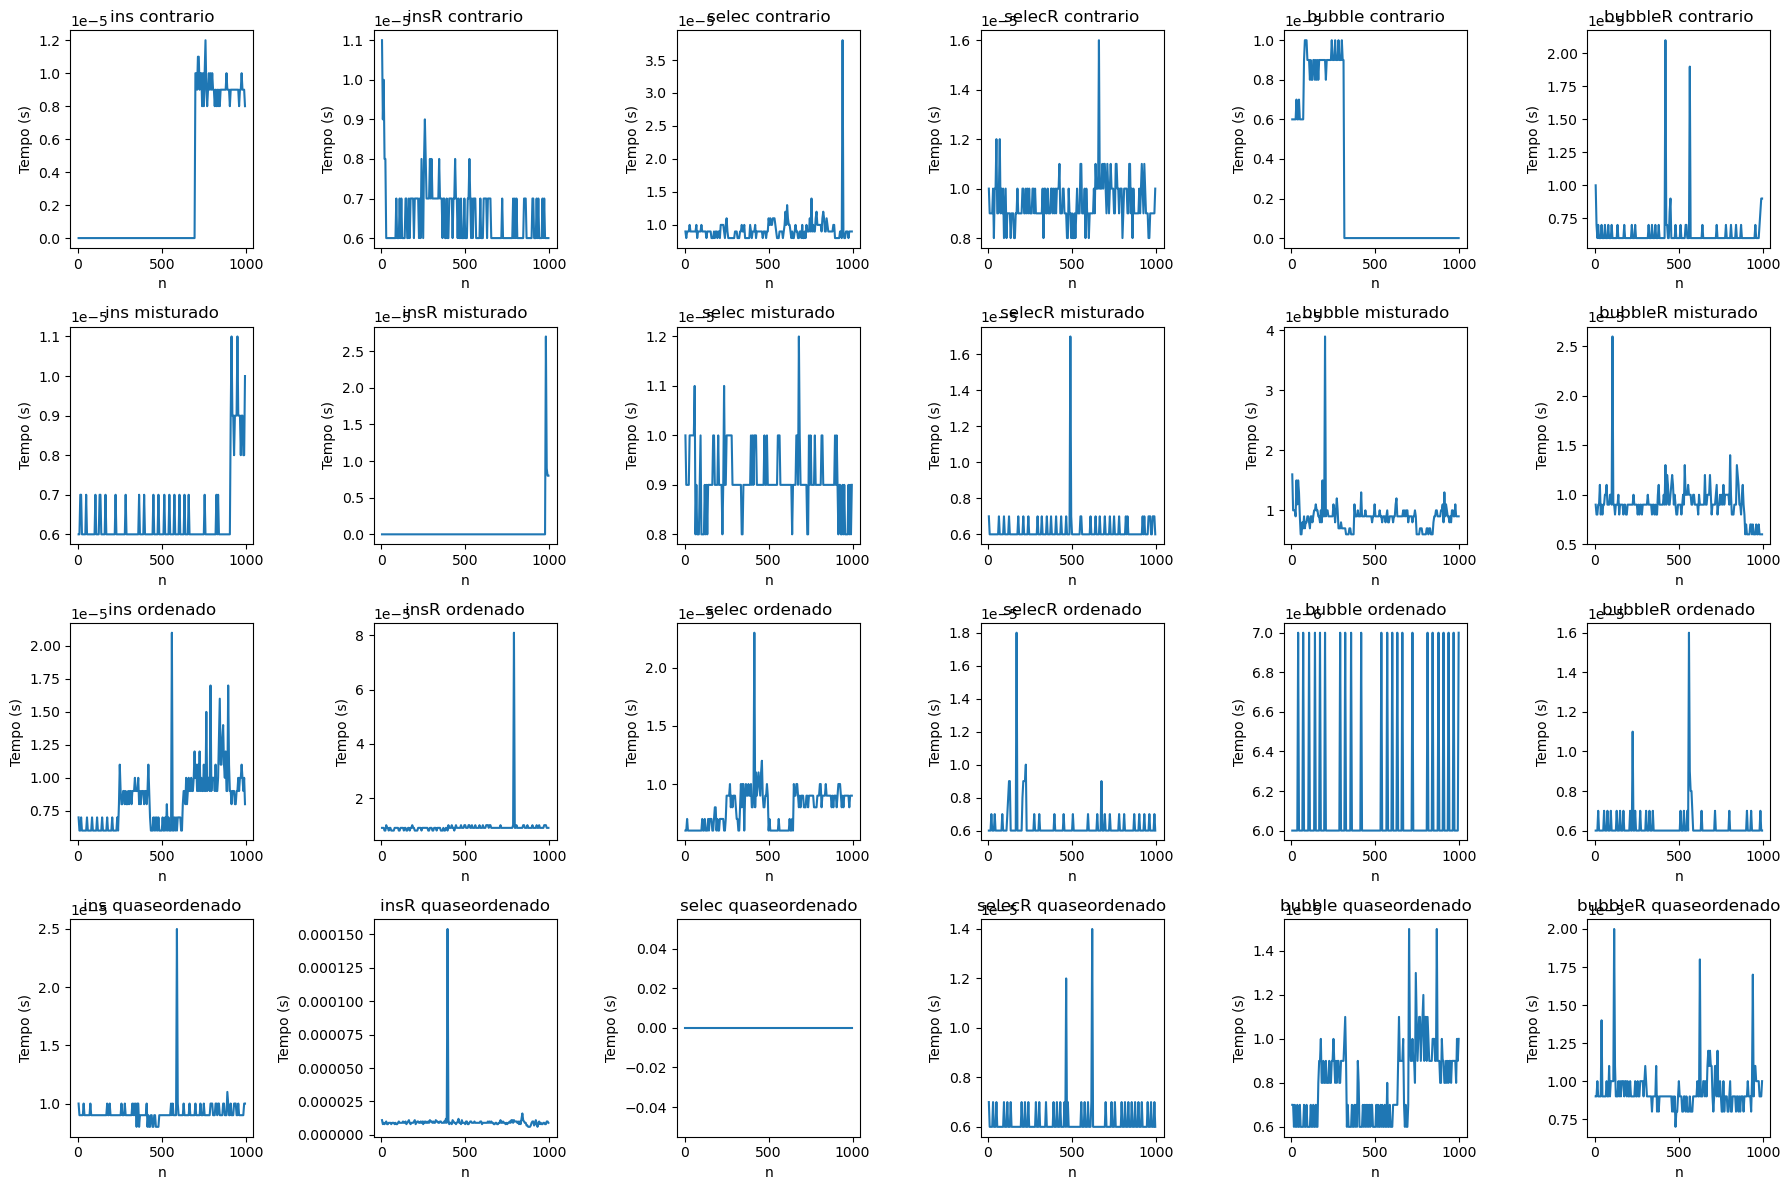
\includegraphics[width=0.8\linewidth]{imgs/deuerrado}
	\caption{Complexidade - Erro}
	\label{fig:deuerrado}
\end{figure}

\section{Struct}

struct Pessoa{
	int idade; 
	char nome[30]; 
}


Sejam Pessoas p1 e p2, temos 

\begin{lstlisting}[language=C]
if(p1->idade >= p2->idade)
	doSomething();

else{
	doOtherThing();
}
\end{lstlisting}

\begin{lstlisting}[language=C]
	if(strcmp(p1->nome, p2->nome) < 0)
		doSomething();
	
	else if(strcmp(p1->nome, p2->nome)) > 0){
		doOtherThing();
	}
\end{lstlisting}
